% Author: Izaak Neutelings (March 2020)
\documentclass[border=3pt,tikz]{standalone}
\usepackage{amsmath} % for \dfrac
\usepackage{bm} % \bm
\usepackage{physics}
\usepackage{tikz,pgfplots}
\usepackage[outline]{contour} % glow around text
\usetikzlibrary{calc}
\usetikzlibrary{decorations.markings}
\usetikzlibrary{arrows.meta}
\tikzset{>=latex} % for LaTeX arrow head
\contourlength{1.6pt}
\usepackage{xcolor}
\colorlet{Bcol}{violet!90}
\colorlet{BFcol}{red!60!black}
\colorlet{veccol}{green!45!black}
\colorlet{Icol}{blue!70!black}
\colorlet{mucol}{red!90!black}
\tikzstyle{BField}=[->,thick,Bcol]
\tikzstyle{current}=[->,Icol] %thick,
\tikzstyle{force}=[->,thick,BFcol]
\tikzstyle{vector}=[->,thick,veccol]
\tikzstyle{mu vector}=[->,thick,mucol]
\tikzstyle{velocity}=[->,very thick,vcol]
\tikzstyle{metal}=[top color=black!15,bottom color=black!25,middle color=black!5,shading angle=20]
\tikzset{
  BFieldLine/.style={thick,Bcol,decoration={markings,mark=at position #1 with {\arrow{latex}}},
                                 postaction={decorate}},
  BFieldLine/.default=0.5,
  ArrowLine/.style={very thick,decoration={markings,mark=at position #1 with {\arrow{latex}}},
                               postaction={decorate}},
  ArrowLine/.default=0.5
}


\begin{document}


% NAIL without field
\def\L{2.0}
\def\T{0.4}
\def\w{0.8}
\def\h{0.3}
\def\l{0.14}
\def\micromu#1#2{
  \draw[mu vector,-{Latex[length=3,width=2]},thin] (\T/2*#1*\L)++(#2-180:\l) --++ (#2:2*\l);
}
\begin{tikzpicture}
  \begin{scope}[rotate=-40]
    \draw[metal]
      (-\T/2,0) --++ (0,\L) -- (-\w/2,\L) --++ (0,\h) --++ (\w,0)
      --++ (0,-\h) -- (\w/2,\L) -- (\T/2,\L) -- (\T/2,0) -- (0,-0.25*\L) -- cycle;
    \micromu{-0.05,-0.10}{-130};
    \micromu{ 0.05,-0.15}{-130};
    \micromu{-0.60, 0.05}{  80};
    \micromu{-0.05, 0.02}{  80};
    \micromu{ 0.60, 0.05}{  80};
    \micromu{-0.55, 0.20}{ 130};
    \micromu{ 0.00, 0.21}{ 130};
    \micromu{ 0.55, 0.22}{ -50};
    \micromu{ 0.65, 0.33}{-100};
    \micromu{-0.20, 0.34}{  15};
    \micromu{ 0.00, 0.40}{  15};
    \micromu{-0.75, 0.50}{-110};
    \micromu{-0.25, 0.51}{-110};
    \micromu{ 0.25, 0.52}{-110};
    \micromu{ 0.75, 0.53}{-110};
    \micromu{-0.20, 0.64}{ 170};
    \micromu{ 0.00, 0.70}{ 170};
    \micromu{ 0.50, 0.80}{  70};
    \micromu{-0.50, 0.82}{ -80};
    \micromu{-0.00, 0.85}{ -80};
    \micromu{ 0.50, 0.95}{ -82};
    \micromu{-0.36, 0.95}{  30};
    \micromu{-0.36, 1.02}{  30};
    %\micromu{-0.36, 1.05}{  30};
    \micromu{-0.95, 1.05}{  30};
    \micromu{-1.40, 1.10}{-130};
    %\micromu{-1.10, 1.11}{-120};
    \micromu{-0.05, 1.12}{-170};
    %\micromu{ 0.90, 1.12}{-170};
    \micromu{ 0.92, 1.06}{ 120};
    \micromu{ 1.55, 1.08}{ 120};
  \end{scope}
\end{tikzpicture}


% NAIL with B FIELD
\begin{tikzpicture}
  \def\NB{4}
  \foreach \i [evaluate={\y=-0.28*\L+(\i-1)*(1.2*\L)/(\NB-1); \f=0.72-0.06*\i;}] in {1,...,\NB}{
    \draw[BFieldLine=\f] (-0.3*\L,\y) --++ (10:1.3*\L);
  }
  \node[Bcol] at (-0.25*\L,0.8*\L) {$\vb{B}$};
  \begin{scope}[rotate=-40]
    \draw[metal]
      (-\T/2,0) --++ (0,\L) -- (-\w/2,\L) --++ (0,\h) --++ (\w,0)
      --++ (0,-\h) -- (\w/2,\L) -- (\T/2,\L) -- (\T/2,0) -- (0,-0.25*\L) -- cycle;
    \draw[mu vector] (0.8*\T,0.78*\L) --++ (50:0.4*\L) node[right] {$\vb*{\mu}_\text{net}$};
    \micromu{ 0.10,-0.18}{50};
    \micromu{ 0.05,-0.11}{50};
    \micromu{ 0.00,-0.05}{50};
    \micromu{-0.50, 0.05}{50};
    \micromu{ 0.00, 0.05}{50};
    \micromu{ 0.50, 0.05}{50};
    \micromu{-0.50, 0.18}{50};
    \micromu{ 0.00, 0.18}{50};
    \micromu{ 0.50, 0.18}{50};
    \micromu{-0.50, 0.31}{50};
    \micromu{ 0.00, 0.31}{50};
    \micromu{ 0.50, 0.31}{50};
    \micromu{-0.50, 0.44}{50};
    \micromu{ 0.00, 0.44}{50};
    \micromu{ 0.50, 0.44}{50};
    \micromu{-0.50, 0.57}{50};
    \micromu{ 0.00, 0.57}{50};
    \micromu{ 0.50, 0.57}{50};
    \micromu{-0.50, 0.70}{50};
    \micromu{ 0.00, 0.70}{50};
    \micromu{ 0.50, 0.70}{50};
    \micromu{-0.50, 0.83}{50};
    \micromu{ 0.00, 0.83}{50};
    \micromu{ 0.50, 0.83}{50};
    \micromu{-0.50, 0.96}{50};
    \micromu{ 0.00, 0.96}{50};
    \micromu{ 0.50, 0.96}{50};
    \micromu{-1.50, 1.08}{50};
    \micromu{-1.00, 1.08}{50};
    \micromu{-0.50, 1.08}{50};
    \micromu{ 0.00, 1.08}{50};
    \micromu{ 0.50, 1.08}{50};
    \micromu{ 1.00, 1.08}{50};
    \micromu{ 1.50, 1.08}{50};

  \end{scope}
\end{tikzpicture}



% DOMAINS
\def\l{0.18*\H}
\def\W{3.6}
\def\H{2.0}
\def\micromu#1#2{
  \draw[mu vector,->] (\W*#1*\H)++(#2-180:\l) --++ (#2:2*\l);
}
\begin{tikzpicture} %[xscale=3.6,yscale=2]
  \coordinate (BL) at (0.25*\W,0.00*\H);
  \coordinate (BR) at (0.70*\W,0.00*\H);
  \coordinate (TL) at (0.40*\W,1.00*\H);
  \coordinate (TR) at (0.80*\W,1.00*\H);
  \coordinate (L)  at (0.00*\W,0.65*\H);
  \coordinate (R)  at (1.00*\W,0.60*\H);
  \coordinate (LT) at (0.25*\W,0.60*\H);
  \coordinate (LB) at (0.30*\W,0.30*\H);
  \coordinate (RT) at (0.65*\W,0.60*\H);
  \coordinate (RB) at (0.72*\W,0.36*\H);
  \draw[metal] (0,0) rectangle (\W,\H);
  \draw (L) to[out=-20,in=-150] (LT) to[out=30,in=-100] (TL);
  \draw (BL) to[out=80,in=-90] (LB) to[out=90,in=-70] (LT);
  \draw (LB) to[out=30,in=-110] (RT) to[out=70,in=-100] (TR);
  \draw (BR) to[out=80,in=-75] (RB) to[out=105,in=-50] (RT);
  \draw (RB) to[out=20,in=-170] (R);
  \micromu{0.15,0.10}{ 17};
  \micromu{0.15,0.22}{ 17};
  \micromu{0.15,0.34}{ 17};
  \micromu{0.14,0.46}{ 17};
  %\micromu{0.12,0.50}{ 17};
  \micromu{0.08,0.80}{100};
  \micromu{0.15,0.78}{100};
  \micromu{0.22,0.80}{100};
  %\micromu{0.30,0.82}{100};
  \micromu{0.35,0.64}{-120};
  \micromu{0.41,0.56}{-120};
  \micromu{0.50,0.58}{-120};
  \micromu{0.60,0.62}{-120};
  \micromu{0.45,0.82}{-120};
  \micromu{0.53,0.82}{-120};
  \micromu{0.61,0.82}{-120};
  \micromu{0.40,0.08}{ 175};
  \micromu{0.42,0.18}{ 175};
  \micromu{0.45,0.28}{ 175};
  \micromu{0.60,0.34}{ 175};
  \micromu{0.61,0.21}{ 175};
  \micromu{0.58,0.10}{ 175};
  \micromu{0.77,0.20}{  75};
  \micromu{0.85,0.22}{  75};
  \micromu{0.93,0.24}{  75};
  \micromu{0.80,0.57}{  -5};
  \micromu{0.84,0.66}{  -5};
  \micromu{0.86,0.76}{  -5};
  \micromu{0.89,0.85}{  -5};
%  \node[scale=0.7] at (BL) {BL};
%  \node[scale=0.7] at (BR) {BR};
%  \node[scale=0.7] at (TL) {TL};
%  \node[scale=0.7] at (TR) {TR};
%  \node[scale=0.7] at (L) {L};
%  \node[scale=0.7] at (R) {R};
%  \node[scale=0.7] at (LT) {LT};
%  \node[scale=0.7] at (LB) {LB};
%  \node[scale=0.7] at (RT) {RT};
%  \node[scale=0.7] at (RB) {RB};
\end{tikzpicture}



% MANY MAGNETIC LOOPS
\def\Rx{1.0}
\def\Ry{0.9}
\def\L{2.4}
\def\ang{120}
\begin{tikzpicture}
  \def\Nr{3}
  \draw[metal] (\ang:{\Rx} and {\Ry}) --++ (\ang-90:\L) arc(\ang:\ang-180:{\Rx} and {\Ry})
    --++ (\ang+90:\L) arc(\ang-180:\ang:{\Rx} and {\Ry});
  \draw[metal] (0,0) ellipse ({\Rx} and {\Ry});
  \foreach \i [evaluate={\r=-0.08+0.9*\i/\Nr; \N=-2+6*\i}] in {1,...,\Nr}{
    \foreach \j [evaluate={\t=\j*360/\N;}] in {1,...,\N}{
      \draw[current,-{Latex[length=2,width=2]}]
        (\t:{\r*\Rx} and {\r*\Ry})++(100:{0.1*\Rx} and {0.1*\Ry}) arc (100:410:{0.1*\Rx} and {0.1*\Ry}) --++ (155:0.07*\Rx);
    }
  }
  %\draw[mu vector] (0.8*\T,0.78*\L) --++ (50:0.4*\L) node[right] {$\vb*{\mu}_\text{net}$};
  
\end{tikzpicture}



% MANY MAGNETIC LOOPS
\begin{tikzpicture}
  \draw[metal] (\ang:{\Rx} and {\Ry}) --++ (\ang-90:\L) arc(\ang:\ang-180:{\Rx} and {\Ry})
    --++ (\ang+90:\L) arc(\ang-180:\ang:{\Rx} and {\Ry});
  \draw[metal] (0,0) ellipse ({\Rx} and {\Ry});
  
  \draw[current,->] %{Latex[length=2,width=2]}
    (70:{0.82*\Rx} and {0.82*\Ry}) arc (70:400:{0.82*\Rx} and {0.82*\Ry}) node[left=4,below=3] {$I$}; %--++ (155:0.07*\Rx);
  %\draw[mu vector] (\ang-160:{1.4*\Rx} and {1.4*\Ry}) --++ (\ang-90:0.6*\L) node[right] {$\vb{M}$};
  \draw[<->] (\ang-170:{1.2*\Rx} and {1.4*\Ry}) --++ (\ang-90:\L) node[midway,fill=white,inner sep=2] {$\ell$};
  
\end{tikzpicture}



% HYSTERESIS
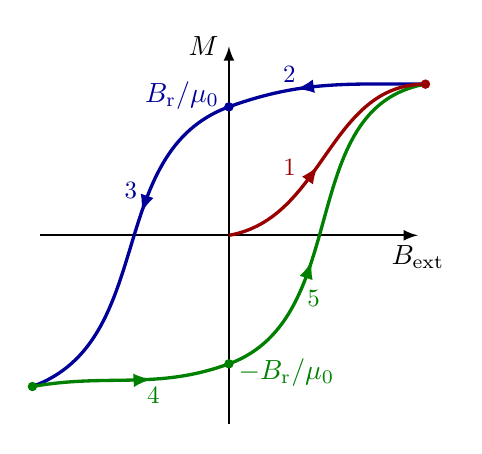
\begin{tikzpicture}
  \def\xmax{2.4}
  \def\ymax{2.4}
  \def\A{0.8*\ymax}
  \def\R{0.06}
  \coordinate (A) at (1.3*\A,\A);
  \coordinate (-A) at (-1.3*\A,-\A);
  \coordinate (T) at (0, 0.85*\A);
  \coordinate (B) at (0,-0.85*\A);
  \draw[->,thick] (0,-\ymax) -- (0,\ymax) node[left] {$M$};
  \draw[->,thick] (-\xmax,0) -- (\xmax,0) node[below] {$B_\text{ext}$};
  \draw[ArrowLine=0.65,blue!60!black] (A) to[out=-180,in=20] (T);
  \draw[ArrowLine=0.40,blue!60!black] (T) to[out=-160,in=20] (-A); %node[midway,above] {$1$};
  \draw[ArrowLine=0.60,green!50!black] (-A) to[out=10,in=-160] (B); %node[midway,left] {$2$};
  \draw[ArrowLine=0.38,green!50!black] (B) to[out=20,in=-170] (A); %node[midway,below] {$3$};
  \draw[ArrowLine=0.45,red!60!black] (0,0) to[out=10,in=-180] (A); %node[midway,right] {$4$};
  \node[left,red!60!black,scale=0.9]    at ( 0.50*\A, 0.45*\A) {$1$};
  \node[above,blue!60!black,scale=0.9]  at ( 0.40*\A, 0.95*\A) {$2$};
  \node[left,blue!60!black,scale=0.9]   at (-0.55*\A, 0.30*\A) {$3$};
  \node[below,green!50!black,scale=0.9] at (-0.50*\A,-0.95*\A) {$4$};
  \node[right,green!50!black,scale=0.9] at ( 0.46*\A,-0.42*\A) {$5$};
  \fill[red!60!black] (A) circle (\R);
  \fill[blue!60!black] (T) circle (\R) node[above=4,left] {$B_\mathrm{r}/\mu_0$};
  \fill[green!50!black] (-A) circle (\R);
  \fill[green!50!black] (B) circle (\R) node[below=3,right] {$-B_\mathrm{r}/\mu_0$};
\end{tikzpicture}


\end{document}